

\documentclass{article}
\usepackage[utf8]{inputenc}
\usepackage[utf8]{inputenc}
\usepackage[T1]{fontenc}
\usepackage[english]{babel}
\usepackage{fullpage}
\usepackage{color}
\usepackage[table]{xcolor}
\usepackage{listings}
 
\definecolor{darkWhite}{rgb}{0.94,0.94,0.94}
 
\lstset{
  aboveskip=3mm,
  belowskip=-2mm,
  backgroundcolor=\color{darkWhite},
  basicstyle=\footnotesize,
  breakatwhitespace=false,
  breaklines=true,
  captionpos=b,
  commentstyle=\color{red},
  deletekeywords={...},
  escapeinside={\%*}{*)},
  extendedchars=true,
  framexleftmargin=16pt,
  framextopmargin=3pt,
  framexbottommargin=6pt,
  frame=tb,
  keepspaces=true,
  keywordstyle=\color{blue},
  language=C,
  literate=
  {²}{{\textsuperscript{2}}}1
  {⁴}{{\textsuperscript{4}}}1
  {⁶}{{\textsuperscript{6}}}1
  {⁸}{{\textsuperscript{8}}}1
  {€}{{\euro{}}}1
  {é}{{\'e}}1
  {è}{{\`{e}}}1
  {ê}{{\^{e}}}1
  {ë}{{\¨{e}}}1
  {É}{{\'{E}}}1
  {Ê}{{\^{E}}}1
  {û}{{\^{u}}}1
  {ù}{{\`{u}}}1
  {â}{{\^{a}}}1
  {à}{{\`{a}}}1
  {á}{{\'{a}}}1
  {ã}{{\~{a}}}1
  {Á}{{\'{A}}}1
  {Â}{{\^{A}}}1
  {Ã}{{\~{A}}}1
  {ç}{{\c{c}}}1
  {Ç}{{\c{C}}}1
  {õ}{{\~{o}}}1
  {ó}{{\'{o}}}1
  {ô}{{\^{o}}}1
  {Õ}{{\~{O}}}1
  {Ó}{{\'{O}}}1
  {Ô}{{\^{O}}}1
  {î}{{\^{i}}}1
  {Î}{{\^{I}}}1
  {í}{{\'{i}}}1
  {Í}{{\~{Í}}}1,
  morekeywords={*,...},
  numbers=left,
  numbersep=10pt,
  numberstyle=\tiny\color{black},
  rulecolor=\color{black},
  showspaces=false,
  showstringspaces=false,
  showtabs=false,
  stepnumber=1,
  stringstyle=\color{gray},
  tabsize=4,
  title=\lstname,
}
\usepackage{graphicx}
\title{HAI819I – Moteurs de jeux
}
\author{Fabien Caballero}

\begin{document}

\maketitle
    \tableofcontents

\newpage
\section{Création du plan}
Pour créer le plan, il nous faut remplir nos buffers de vertices et d'indices de triangles, pour cela on doit remplir deux vector (indexed\_vertices et indices).
Pour cela j'ai créé une fonction makePlan, qui prends en paramètres la résolution, le décalage par rapport au centre et la taille horizontale et verticale.
Pour créer les vertices on fait une double boucle for dont la première fait resX+1 itérations, avec resX la résolution horizontale et la deuxième pareil mais avec la resolution verticale.
Cela car pour une resolution de 1 par 1 on a 4 points pour former un carré, d'où (resolutionH+1)*(resolutionV+1) points.
Pour chaque itérations, on ajoute dans notre liste de points (indexed\_vertices) un nouveau vecteur qui a pour coordonnées:

x = (taille\_horizontale/resolutionH) *cptPremièreBoucle  ici on prend la taille horizontale du plan qu'on divise par la résolution horizontale ainsi on obtient le décalage horizontal entre chaques points et on multiplie par le compteur de notre première boucle pour placer le point au bon endroit sur l'axe X 
\\\\
y =  on le défini à 0 pour avoir un plan parfaitement plat
\\\\
z = (taille\_verticale/resolutionV) *cptDeuxièmeBoucle  ici on prend la taille verticale du plan qu'on divise par la resolution verticale ainsi on obtient le décalage vertical entre chaques points et on multiplie par le compteur de notre deuxième boucle pour placer le point au bon endroit sur l'axe Z 

Ensuite dans 2 autres boucles à part, cette fois-ci allant de 0 à resolutionH-1 et de 0 à resolutionV-1, on va créer nos indices de triangles.
pour cela à chaque itération on vas créer 2 triangles, le triangle inférieur et supérieur d'un carré.
\begin{figure}[h!]
\centerline{ \includegraphics[scale=0.5]{./rendus/schéma1.png} }
\caption{schéma du triangle supérieur et inférieur d'un carré} 
\end{figure}

Étant donné qu'il faut récupérer l'indice du bon sommet on utilise notre premier compteur qu'on multiplie par resolutionH et on y additione le deuxième compteur.
Cela revient à un parcours linéaire d'une matrice de sommets, stockée dans un tableau. 

On ajoute nos 6 indices correspondant aux 3 sommets des 2 triangles en utilisant cette méthode.

À la fin de la fonction on génère et ont rempli les 2 buffers avec indexed\_vertices et indices complétés précédemment.
\newpage


On obtient le résultat ci-dessous:
\begin{figure}[h!]
\centerline{ 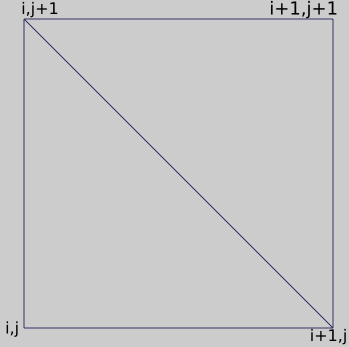
\includegraphics[scale=0.5]{./rendus/plan1.png} 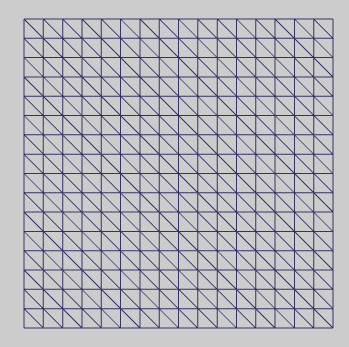
\includegraphics[scale=0.5]{./rendus/plan.png} }
\caption{plan avec une resolution de 1 et de 16} 
\end{figure}

J'ai utilisé des paramètres supplémentaires offSetX et offSetZ qui me permettent de bouger mon plan selon l'axe X et Z.

\newpage
\section{Plaquer une texture}
Pour plaquer une texture  il faut load une texture avec la fonction loadBMP\_custom ou loadTexture2DFromFilePath (qui utilise stbi\_load) on envoie cette texture au fragment shader. Dans celui-ci on ajoute un paramètre uniform sampler2D texture qui sera la texture que l'on a load.
On a maintenant les données il nous faut les coordonnées de textures, pour notre plan il s'agit de 2 paramètres le u et le v on fait le même principe que pour les vertices précédemment. On créé donc un nouveau buffer et pour chaque vertices créées on ajoute dans notre tableau de coordonnées de texture: 
\\\\
u= (1/resolutionH)*cptPremièreBoucle il s'agit du x des vertices mais sans la taille du plan
\\\\
v=(1/resolutionV)*cptDeuxièmeBoucle il s'agit du y des vertices mais sans la taille du plan

On génère notre buffer on le rempli et on envoi au vertex shader, celui-ci l'envoi au fragment qui grâce à la fonction texture ainsi que le sampler2D texture et le vec2 uv on obtient le texel à plaquer sur le fragment de notre plan.

\begin{figure}[h!]
\centerline{ 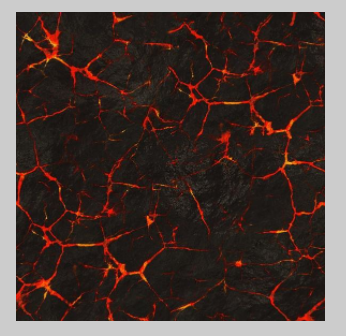
\includegraphics[scale=0.5]{./rendus/text.png} }
\caption{texture lava} 
\end{figure}

Pour avoir des positions aléatoires il suffit lors de la création de nos vertices définir un y aléatoire.

\begin{figure}[h!]
\centerline{ 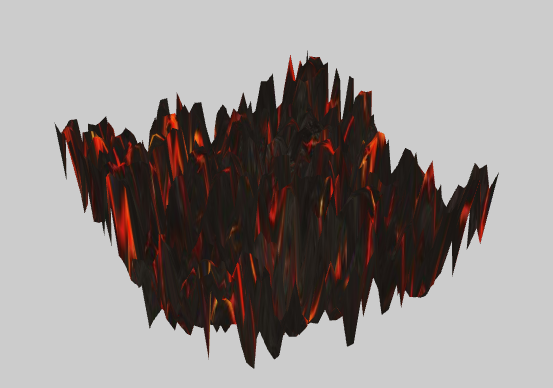
\includegraphics[scale=0.4]{./rendus/rrandom.png} }
\caption{texture lava} 
\end{figure}

\newpage
\section{HeightMap}

Pour réaliser la heightMap il suffit créer une texture à partir de notre image, on l'envoie au vertexShader et celui-ci récupère la valeur de la heightMap grâce aux coordonnées textures et l'utilise en tant que y du sommet.


\begin{figure}[h!]
\centerline{ 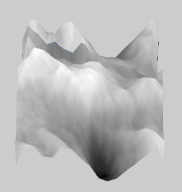
\includegraphics[scale=1]{./rendus/heightmap2.png} 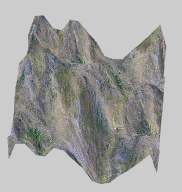
\includegraphics[scale=1]{./rendus/heightmap1.png} }
\caption{height map} 
\end{figure}

\newpage
\section{HeightMap MultiTexturing}

Pour faire le MultiTexturing on charge toutes les textures dont on a besoin puis on active chaque textures on envoie chaque textures au bon sampler2D (avec la fonction glUniform1i), sans oublier de changer le numéro de texture.
Puis on passe en paramètre supplémentaire les seuils qui nous permettront de gérer quand est ce qu'on utilise telle ou telle texture.
 
Ensuite dans le vertex\_shader on calcule notre y avec la heightMap puis on envoi au fragment shader nos seuils ainsi que le y trouvé et en fonction on applique telle ou telle texture.

\begin{figure}[h!]
\centerline{ 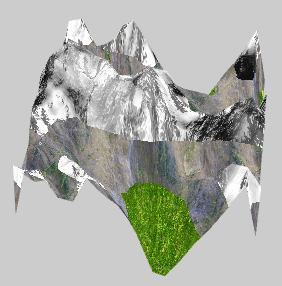
\includegraphics[scale=1]{./rendus/heightmpamultitext.png} }
\caption{height map} 
\end{figure}

\newpage
Afin d'avoir plusieurs mode j'ai défini 3 booléens qui représente l'état de chaque mode et la touche "c" permettant de changer entre libre et orbital et "p" qui permet de se mettre en mode présentation. 

\section{Mode présentation}
Pour avoir un angle de vue de 45° j'ai décaler mis la même valeur en z qu'en y ainsi en définissant ma caméra avec pour cible le centre de mon objet, celle-ci regarde l'objet avec un angle de 45°.
Pour que l'objet tourne sur lui-même, pour chaque frame avant d'actualiser la valeur de la matrice model j'ai effectué une rotation d'une certaine valeur selon l'axe Y ainsi l'objet est tourné à chaque frame, avec des contrôles de touches (UP et DOWN pour mon tp) on peut changer la valeur utilisée dans la rotation et ainsi augmenter la vitesse de rotation.

Voir vidéo ModePresentation.mp4

\section{Mode Libre}

Pour le mode libre:

- afin de se déplacer en avant (avec Z) on ajoute a notre position le vecteur front de la caméra 

- afin de se déplacer en arrière (avec S) on substitue a notre position le vecteur front de la caméra 

- afin de se déplacer sur la droite (avec D) on ajoute a notre position le vecteur right, obtenu en faisant le produit vectoriel entre le vecteur front et up de la caméra

- afin de se déplacer sur la gauche (avec Q) on ajoute a notre position le vecteur right, obtenu en faisant le produit vectoriel entre le vecteur front et up de la caméra
\\\\
Pour que le déplacement soit plus fluide on normalise chaque vecteur résultants et on utilise un flottant permettant de gérer la vitesse de déplacement
\\\\
Voir vidéo ModeLibre.mp4

\section{Mode Orbital}
- afin de se déplacer en avant (avec Z) on ajoute a notre position le vecteur up de la caméra 

- afin de se déplacer en arrière (avec S) on substitue a notre position le vecteur up de la caméra 

- afin de se déplacer sur la droite (avec D) on ajoute a notre position le vecteur right orbital, obtenu en faisant le produit vectoriel entre le vecteur direction (target-position) et up de la caméra

- afin de se déplacer sur la gauche (avec Q) on ajoute a notre position le vecteur right orbital, obtenu en faisant le produit vectoriel entre le vecteur direction (target-position) et up de la caméra
\\\\
Pour que le déplacement soit plus fluide on normalise chaque vecteur résultants et on utilise un flottant permettant de gérer la vitesse de déplacement
\\\\
Voir vidéo ModeOrbital.mp4


\end{document}